%% LyX 2.4.4 created this file.  For more info, see https://www.lyx.org/.
%% Do not edit unless you really know what you are doing.
\documentclass[english]{article}
\usepackage[T1]{fontenc}
\usepackage[latin9]{inputenc}
\usepackage{float}
\usepackage{enumitem}
\usepackage{amsmath}
\usepackage{amsthm}
\usepackage{cancel}
\usepackage{geometry}
\geometry{verbose,tmargin=1in,bmargin=1in,lmargin=1in,rmargin=1in}

\makeatletter

%%%%%%%%%%%%%%%%%%%%%%%%%%%%%% LyX specific LaTeX commands.
%% Because html converters don't know tabularnewline
\providecommand{\tabularnewline}{\\}

%%%%%%%%%%%%%%%%%%%%%%%%%%%%%% Textclass specific LaTeX commands.
\numberwithin{equation}{section}
\numberwithin{figure}{section}
\newlength{\lyxlabelwidth}      % auxiliary length 

%%%%%%%%%%%%%%%%%%%%%%%%%%%%%% User specified LaTeX commands.
\usepackage{hyperref}
\usepackage[usenames,dvipsnames,table]{xcolor} %adds additional color options
\hypersetup{colorlinks=true, urlcolor=black,linkcolor=black}

\usepackage{fancyhdr}
\usepackage{lastpage}
\pagestyle{fancy}
\usepackage{enumitem}
\usepackage{ifthen}
%sets math fonts to be more readable
\everymath=\expandafter{\the\everymath\displaystyle}
%\DeclareMathSizes{10}{10}{10}{10}
\usepackage{multicol}

\usepackage{tikz}
\usetikzlibrary{plotmarks}
\usepackage{pgfplots}
\pgfplotsset{compat=newest}

\usepackage{calc}
\usepackage[nomessages]{fp}

\usepackage{advdate}    % Advancing/saving dates
\usepackage{datetime}   % Dates formatting
\usepackage{datenumber} % Counters for dates

\usepackage{fancybox} %%ovalbox and fancy box settings

\usepackage[super]{nth} %easy 1st, 2nd, etc

\usepackage{forest} %%for tree diagram

%%data for histogram%%
\begin{filecontents}{hist1_data.csv} 
dist 
3
1
0
4
1
3
2
2
0
2
0
2
2
1
4
3
1
1
3
4
2
1
3
0
1
0
2
5
1
2
3
0
0
1
2
3
1
2
0
2
\end{filecontents}

%%data for histogra: cal per cereal%%
\begin{filecontents}{hist_data_cereal.csv} 
dist 
3.7
3.6
3.6
4.0
4.0
3.6
3.8
3.7
4.1
3.9
3.9
3.3
3.5
3.6
3.9
4.0
\end{filecontents}
% Added by lyx2lyx
\setlength{\parskip}{\smallskipamount}
\setlength{\parindent}{0pt}

\makeatother

\usepackage{babel}
\begin{document}
\renewcommand{\author}{Dr.\,James Ashe}

\newcommand{\classNum}{107}

\newcommand{\classSec}{7 and 10}

\newcommand{\nameType}{}

\newcommand{\examType}{Exam 4 Review}

\renewcommand{\date}{Exam 4 is on \formatdate{21}{11}{2014}}

%%First page's header%%%%%%%%%%%%%%%%%%%%%%
\fancypagestyle{firststyle} %%header settings for first pagr
{
	\fancyhead[L]{MTH \classNum{}(\classSec{}) \author{}\\
	\textbf{\examType{}} \date{}}
	\fancyhead[C]{\textbf{\nameType}}
	\setlength{\headsep}{14pt}
}
%%%%%%%%%%%%%%%%%%%%%%%%%%%%%%%%%%%%%%%%%%

%%Next page's header%%%%%%%%%%%%%%%%%%%%%%%
%\setlist{nolistsep}
\lhead{MTH \classNum{}(\classSec{})} 
\chead{\textbf{\nameType}} 
\cfoot{\thepage{}~of~\pageref{LastPage}} 
\setlength{\headsep}{5pt} 
%%%%%%%%%%%%%%%%%%%%%%%%%%%%%%%%%%%%%%%%%%%

%%Various settings; see the preamble for other settings%%%%%
%%\setenumerate[0]{leftmargin=12pt,itemindent=0pt,labelwidth=0pt}
%\setlist[2]{noitemsep}
%\setlist{nosep}
\setlist{itemsep=-3pt,topsep=-2pt}
\renewcommand{\labelenumi}{\textbf{\arabic{enumi}.}}
\renewcommand{\labelenumii}{\textbf{\alph{enumii}.}}
\thispagestyle{firststyle}
%%%%%%%%%%%%%%%%%%%%%%%%%%%%%%%%%%%%%%%%%%
\newcommand{\xmax}{10}
\newcommand{\xmin}{-10}
\newcommand{\xstep}{0} %must be xmin+n
\newcommand{\ymax}{10}
\newcommand{\ymin}{-10}
\newcommand{\ystep}{0} %must be ymin+n

\newcommand{\xspace}{\hspace*{40pt}}
\newcommand{\yspace}{\vspace*{1.4cm}}
\newcommand{\rowColor}{gray!35}
\large

\emph{Unless stated otherwise, all problems are worth equal value
and answers should be stated as decimals rounded to three decimal
places. You must show your work to receive credit. }
\begin{enumerate}[resume]
\item Use figure \ref{fig:Number-of-children} to complete the following.\begin{multicols}{2}

\begin{enumerate}
\item Create a frequency distribution from figure \ref{fig:Number-of-children}
(approximate the values as best as possible).\vfill
\item Find the mean weight of cereal boxes.\vfill
\item Find the mode weight of cereal boxes. \vfill
\item Is the data normally distributed?\vfill\columnbreak
\item []
\begin{figure}[H]
\begin{centering}
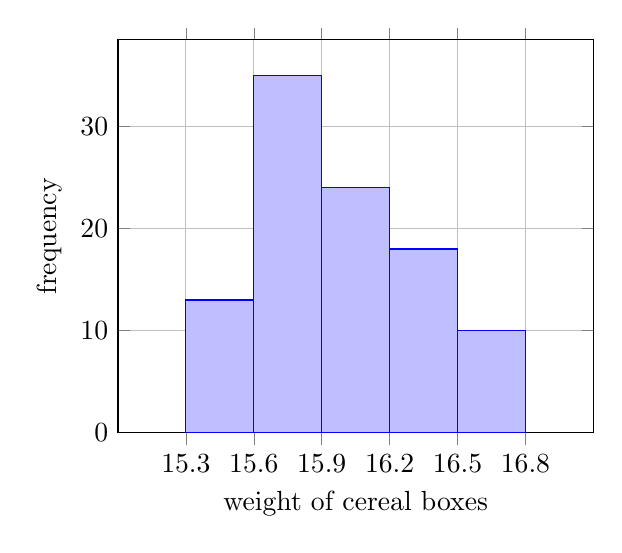
\begin{tikzpicture}[scale=1]
\begin{axis}[     
	ybar interval,
	x tick label as interval=false,    
	ymin=0,
	xmin=15,
	xmax=17.1,
	width=3in,
	%height=3in,
	grid=major,
	ylabel=frequency,
	xlabel=weight of cereal boxes
	] 
	\addplot [fill=blue!25,draw=blue] table [x=Lower, y=Count] { 
		Lower Upper Count 
		15.3 15.6 13
		15.6 15.9 35
		15.9 16.2 24
		16.2 16.5 18
		16.5 16.8 10
		16.8 17.1 0
	};
\end{axis}
\end{tikzpicture}
\par\end{centering}
\caption{\label{fig:Number-of-children}Weights of boxes of cereal.}
\end{figure}
\yspace\yspace
\end{enumerate}
\end{multicols}
\item Forty randomly selected families were surveyed to determine the number
of children in each family. The following results were found:

\hfill%
\begin{tabular}{cccccccc}
3.7  & 3.6 & 4.0 & 3.8 & 4.1 & 3.9 & 3.5 & 3.9\tabularnewline
3.6 & 4.0 & 3.6 & 3.7 & 3.9 & 3.3 & 3.6 & 4.0\tabularnewline
\end{tabular}\hfill\hspace{0cm}\begin{multicols}{2}
\begin{enumerate}
\item Find the mean.\yspace
\item Find the median.\yspace
\item Find the standard deviation.\yspace 
\item Construct a histogram using 5 subintervals, beginning at 3.2, and
ending at 4.2.\columnbreak
\item []\vspace{4cm}%\begin{tikzpicture}[scale=.8]
%\begin{axis}[     ybar,     ymin=0 ] 
%\addplot +[hist={bins=5,data min=3.2,data max=4.2}] table [y index=0] {hist_data_cereal.csv}; 
%\end{axis} 
%\end{tikzpicture} 
\end{enumerate}
\end{multicols}\newpage
\item Tom and Jerry golfed five times during their vacation. Their scores
are given in the table below:

\hfill%
\begin{tabular}{cccccc}
\textbf{Tom}  & 103 & 99 & 107 & 93 & 92\tabularnewline
\textbf{Jerry} & 101 & 92 & 83 & 96 & 111\tabularnewline
\end{tabular}\hfill\hspace{0cm}
\begin{enumerate}[resume]
\item []Who is the more consistent golfer?\yspace\vfill
\end{enumerate}
\item A population is normally distributed with mean 78 and standard deviation
7.5.

\begin{enumerate}
\item Draw a sketch of the bell curve labeling the mean and the intervals
representing 1, 2, and 3 standard deviations of the mean.\yspace\yspace
\item Find the percentage of data lies in each of the intervals.\yspace
\end{enumerate}
\item Find the following probabilities, 

\begin{enumerate}
\item $p(z<1.35)$\yspace\vfill
\item $p(0<z<2.02)$\yspace\vfill
\item $p(-.09<z<1.06)$\yspace\vfill
\item $p(-1.1<z<-.08)$\yspace\vfill\newpage
\end{enumerate}
\item A population is normally distributed with a mean 78 and standard deviation
7.5. Find the following probabilities. 

\begin{enumerate}
\item $p(x<70)$\yspace\vfill
\item $p(70<x<85)$\yspace\vfill
\item $p(80<x<95.5)$\yspace\vfill
\item $p(95.5<x<108)$\yspace\vfill
\end{enumerate}
\item Find $c$ such that each of the following is true.

\begin{enumerate}
\item $p(z<c)=27.76\%$\yspace\vfill
\item $p(z>c)=3.51\%$\yspace\vfill
\item $p(-c<z<c)=73.3\%$\yspace\vfill
\item Let $\mu=100$ and $\sigma=15$ find $c$ such that $p(x<c)=27.76\%$\yspace\vfill
\end{enumerate}
\item The time it takes latex paint to dry is normally distributed with
$\mu=3.5$ hours and $\sigma=.75$ hours. Find the probability that
drying time will be as follows.

\begin{enumerate}
\item less than $2.25$ hours.\yspace\vfill
\end{enumerate}
\item The average score on the ACT is $18$ with a standard deviation of
$6$. If a college only wants to accept students with at least an
ACT score in the top 25\%. What is the minimum score they should accept?
What about the top 5\%?\yspace\vfill
\end{enumerate}

\end{document}
